\documentclass[9pt]{beamer}

\usepackage[T1]{fontenc}
\usepackage{color}
\usepackage{graphicx}
\usepackage{natbib}
\usepackage{tikz}
\usepackage{xmpmulti}
\usepackage{animate}
\usepackage{hyperref}

\usetheme{Boadilla}

\usefonttheme{professionalfonts}

\title[Apsis Tools]{Apsis - Document Review Platform}
\subtitle{}
\author{Max Callaghan}
\institute[MCC]{
	%
\includegraphics[height=1cm,width=2cm]{/home/max/Pictures/MCC_Logo_RZ_rgb.jpg}
	
\includegraphics[height=1cm,width=2cm]{MCC_Logo_RZ_rgb.jpg}
}

\usetikzlibrary{shapes.geometric, arrows}
\tikzstyle{startstop} = [rectangle, rounded corners, minimum width=2.5cm, minimum height=1cm,text centered, draw=black, text width=2.5cm, fill=red!30]
\tikzstyle{placeholder} = [rectangle, rounded corners, minimum width=2.5cm, minimum height=1cm,text centered, draw=white, text width=2.5cm, fill=red!00]
\tikzstyle{product} = [rectangle, rounded corners, minimum width=2.5cm, minimum height=1cm,text centered, draw=black, text width=2.5cm, fill=cyan!30]
\tikzstyle{process} = [rectangle, minimum width=2cm, text width=2cm, minimum height=1cm, text centered, draw=black, fill=orange!30]
\tikzstyle{person} = [ellipse, minimum width=2cm, text width=2cm, minimum height=1cm, text centered, draw=black, fill=green!30]
\tikzstyle{io} = [trapezium, trapezium left angle=70, trapezium right angle=110, minimum width=1cm, minimum height=1cm, text centered, draw=black, fill=blue!30, inner sep=10]

\tikzstyle{label} = [rectangle, minimum width=0.8cm, minimum height=0.8cm, text centered, draw=black, fill=blue!0, inner sep=3]

\tikzstyle{arrow} = [thick,-,>=stealth]
\tikzstyle{darrow} = [dotted, thick,-,>=stealth]

\newtheorem*{remark}{}

\bibliographystyle{apalike}

\begin{document}
	
\begin{frame}
	\titlepage
\end{frame}

\addtobeamertemplate{frametitle}{}{%
	\begin{tikzpicture}[remember picture,overlay]
	\node[anchor=north east,yshift=2pt] at (current page.north east) {
\includegraphics[height=0.8cm]{MCC_Logo_RZ_rgb.jpg}};
	\end{tikzpicture}}

\begin{frame}{Background}
The exponential growth in literature about climate change raises challenges for environmental assessments:
\begin{columns}
	\begin{column}{0.5\linewidth}
		\begin{figure}
			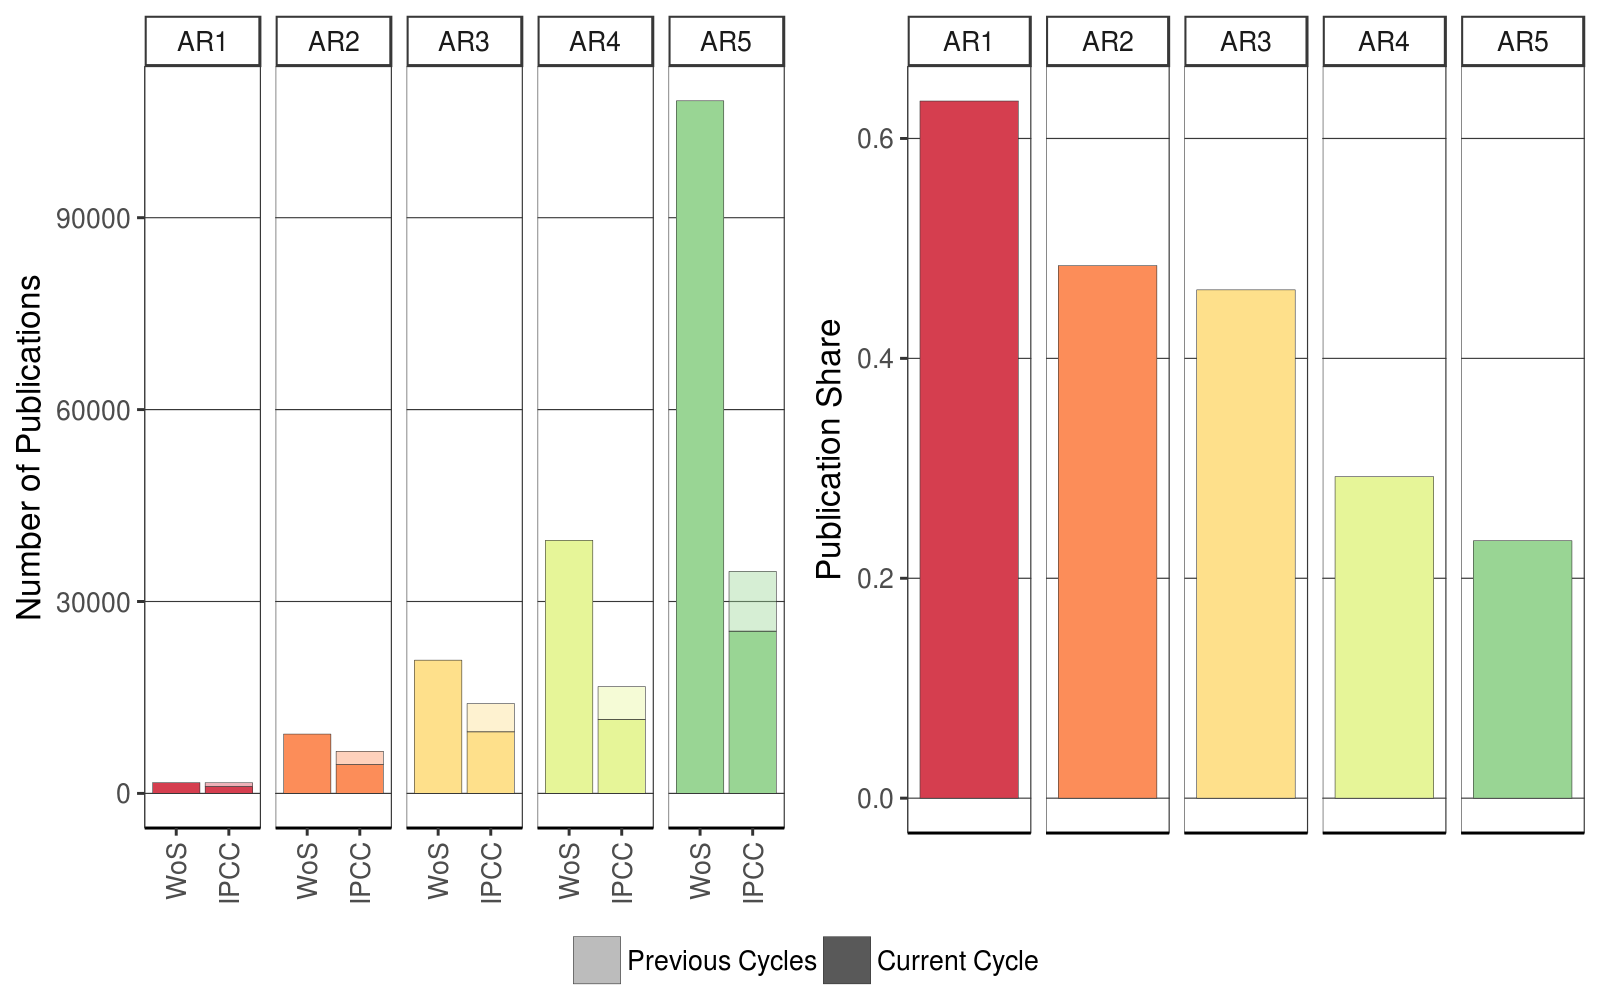
\includegraphics[width=\linewidth]{images/merged_IPCC_spectral}
			\caption{\citep{Minx2017l}}
		\end{figure}
	\end{column}
	\begin{column}{0.5\linewidth}
		\begin{itemize}
			\item<2-> We need to develop ways of being more systematic in engaging with the literature
			\item<3-> We need more research on research results
			\item<4-> We need ways of engaging with large amounts of text
		\end{itemize}
	\end{column}
\end{columns}
\end{frame}

\begin{frame}{Background}

	\begin{figure}
		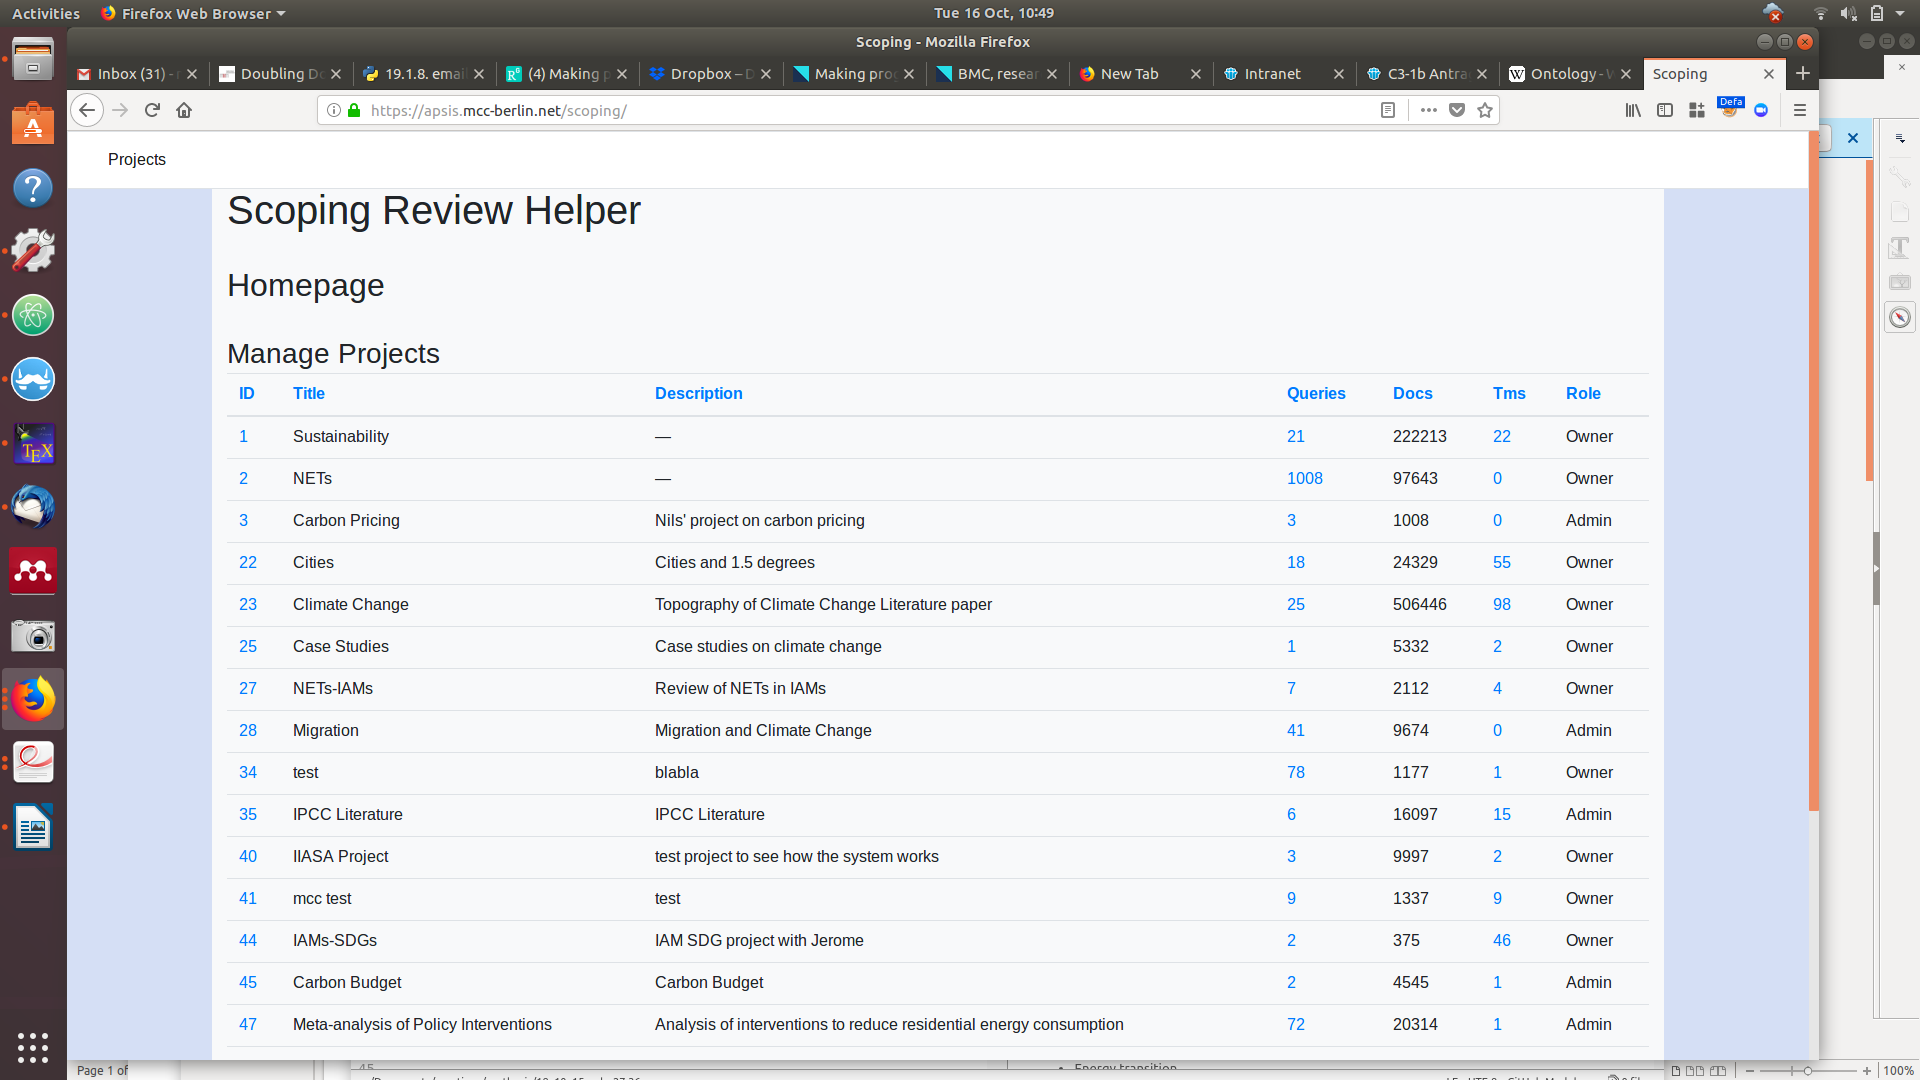
\includegraphics[width=\linewidth]{images/homepage}
	\end{figure}

\end{frame}

\begin{frame}{Infrastructure Overview}
\begin{center}
	\def\yspace{1.5cm}
	\resizebox{0.9\linewidth}{!}{
		\begin{tikzpicture}[node distance=3cm]
		\node (Data) [startstop] {Data Collection};
		\node (Analysis) [startstop, right of=Data, node distance=6cm] {Analysis};
		\node (Presentation) [startstop, right of=Analysis, node distance=6cm] {Outputs};
		
		\node (WoS) [process, below of=Data, node distance=1.8cm, xshift=-2cm] {WoS};
		\node (Scopus) [process, below of=WoS, node distance=\yspace] {Scopus};
		\node (IPCC) [process, below of=Scopus, node distance=\yspace, fill=orange!10] {IPCC};
		\node (Consolidation) [io, right of=Scopus, node distance=3.5cm] {Consolidation};
		
		\node (Manual) [label, below of=Analysis, node distance=1.8cm, xshift=-1.2cm] {Manual};
		\node (Automatic) [label, below of=Manual, node distance=4.5cm] {Automatic};
		
		
		\node (Review) [process, below of=Analysis, node distance=1.8cm, xshift=1cm] {Systematic Review};
		\node (Scientometric) [process, below of=Review, node distance=\yspace, fill=orange!10] {Scientometric Analysis};
		\node (Text) [process, below of=Scientometric, node distance=\yspace, fill=orange!10] {Other Text Analysis};
		\node (Topics) [process, below of=Text, node distance=\yspace] {Topic Modelling};
		
		\node (Plots) [process, below of=Presentation, node distance=1.8cm, xshift=0cm, fill=orange!10] {Plots};
		\node (Tables) [process, below of=Plots, node distance=\yspace] {Tables};
		\node (Online) [process, below of=Tables, node distance=\yspace] {Online Explorer};	
		
		\draw [arrow, ->] (Manual) -- (Automatic);
		
		\end{tikzpicture}
	}
\end{center}

\end{frame}

%%%%%%%%%%%%%%%%%%%%%%%%%%%%%%%%%%%%%%%%%%%%%%%%%%%%% 
%% Systematic review of NETs



\begin{frame}{Systematic Review - NETs}

For our systematic review of NETs, we wanted to be as systematic in our search, selection and treatment of literature as possible. We developed a system to help us

\begin{columns}
	\begin{column}{1\linewidth}
		\begin{itemize}
			\item To search and download (bulk) metadata from Web of Science (WoS) and Scopus
			\item To combine, compare and manage these queries and the documents associated with them
			\item To manage (centrally) the screening of documents by internal and external collaborators
			\item To run analysis based on user-entered tagging of documents and metadata from the WoS/Scopus
		\end{itemize}
	\end{column}

\end{columns}

\end{frame}


%%%%%%%%%%%%%%%%%%%%%%%%%%%%
%% Sys review process

\begin{frame}{Systematic Review - NETs}
\begin{columns}
	\begin{column}{0.5\linewidth}<1->
		We downloaded over 400 queries, and a team of 18 users reviewed hundreds of documents each.
		\begin{figure}
			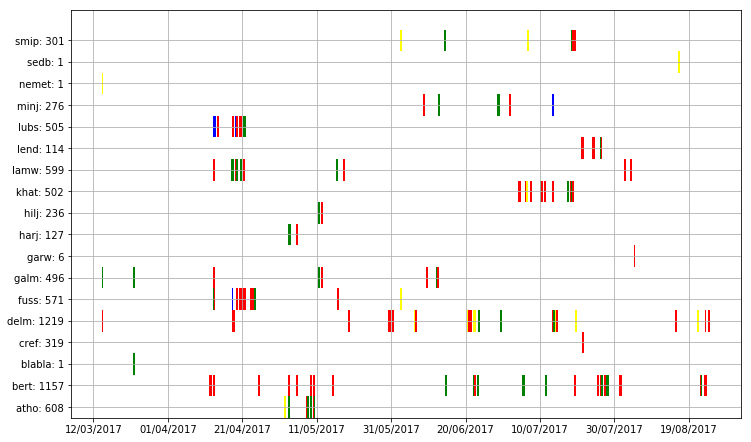
\includegraphics[width=1\linewidth]{images/ratings_user_time}
		\end{figure}
	\end{column}
	\begin{column}{0.5\linewidth}<2->
		\bigskip
		\bigskip
		
		We used the results to automatically email all authors of relevant documents
	\begin{figure}
		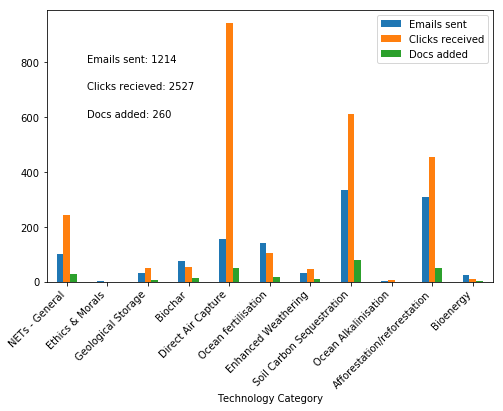
\includegraphics[width=1\linewidth]{images/emails_responses}
	\end{figure}
	\end{column}
\end{columns}

\end{frame}



\begin{frame}{Systematic Review - NETs}
\begin{columns}
	\small
	\begin{column}{0.5\linewidth}<1->
		Based on the labels, we could efficiently characterise this bibliographic coupling network 
	\begin{figure}
		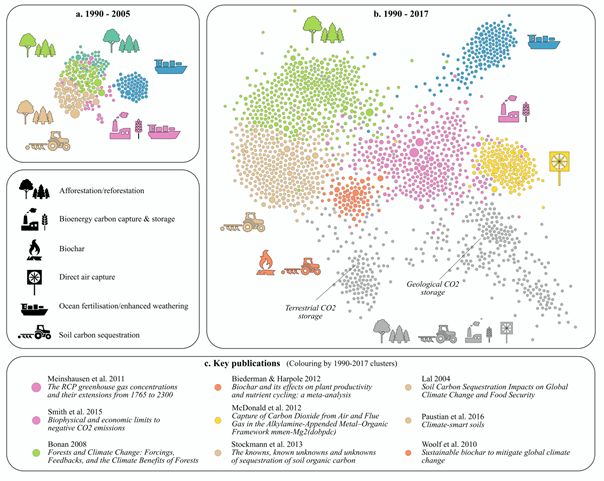
\includegraphics[width=\linewidth]{images/NETs_network}
		\caption{\citep{Minx2018}}
	\end{figure}
	\end{column}
	\begin{column}{0.5\linewidth}
		\begin{itemize}
			\itemsep-1em
			\item[]<2-> And after collecting further information, we could characterise the documents
			\begin{figure}
				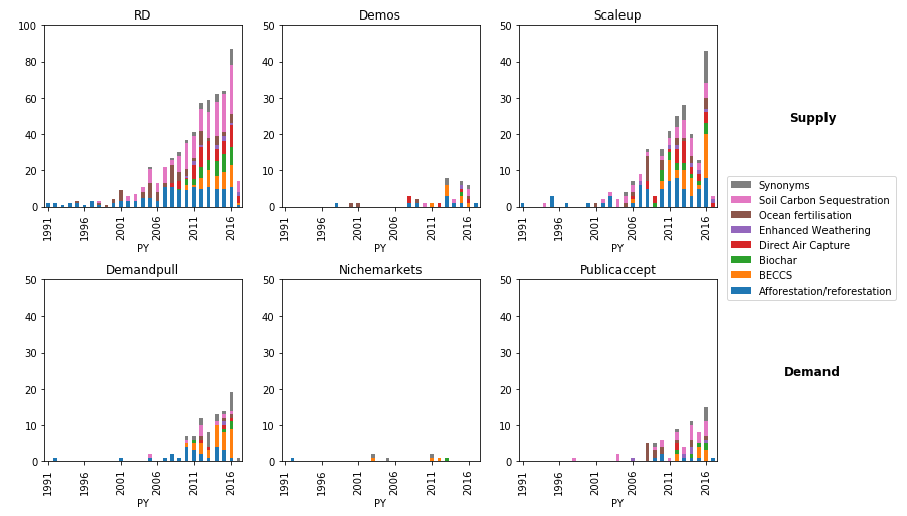
\includegraphics[width=0.8\linewidth]{images/nets_3}
				\caption{\citep{Nemet2018}}
			\end{figure}
			\item[]<3-> And summarise information from them
			\begin{figure}
				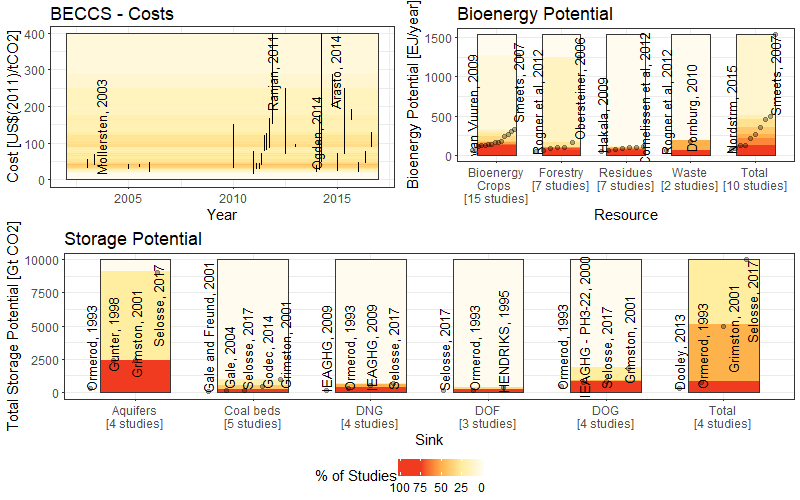
\includegraphics[width=0.8\linewidth]{images/panel}
				\caption{\citep{Fuss2018}}
			\end{figure}	
		\end{itemize}	
	\end{column}
\end{columns}

\end{frame}

%%%%%%%%%%%%%%%%%%%%%%%%%%%%
%% Other projects

\begin{frame}[t]{Other projects}

\normalsize

\begin{columns}[t]
	\begin{column}{0.33\linewidth}
		\centering \textbf{ IAMs \& SDGs with IIASA}
		\begin{figure}
			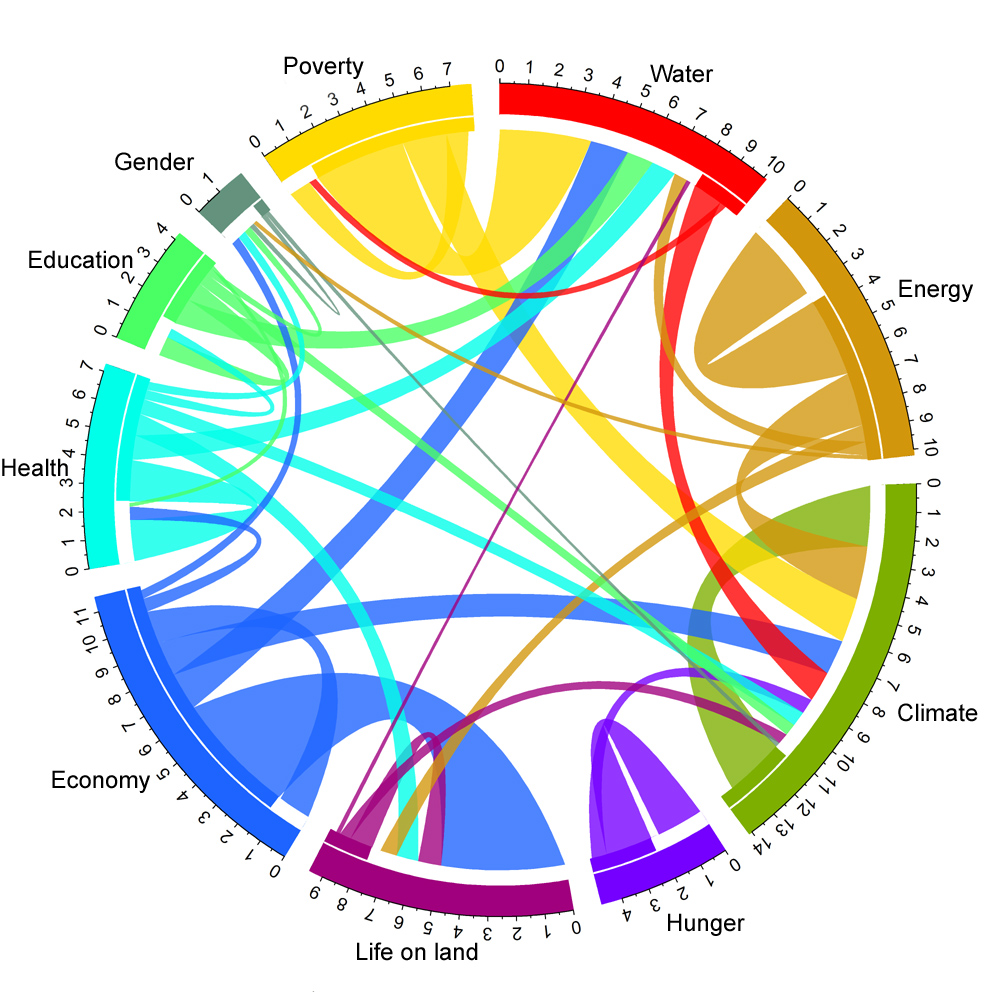
\includegraphics[width=\linewidth]{images/wheel}
		\end{figure}
		\begin{itemize}
			\item colleagues from IIASA now trialling tool
		\end{itemize}
	\end{column}
	\begin{column}{0.33\linewidth}
		\centering \textbf{My PhD work}
		
		+ additional APSIS projects
		
		\begin{figure}
			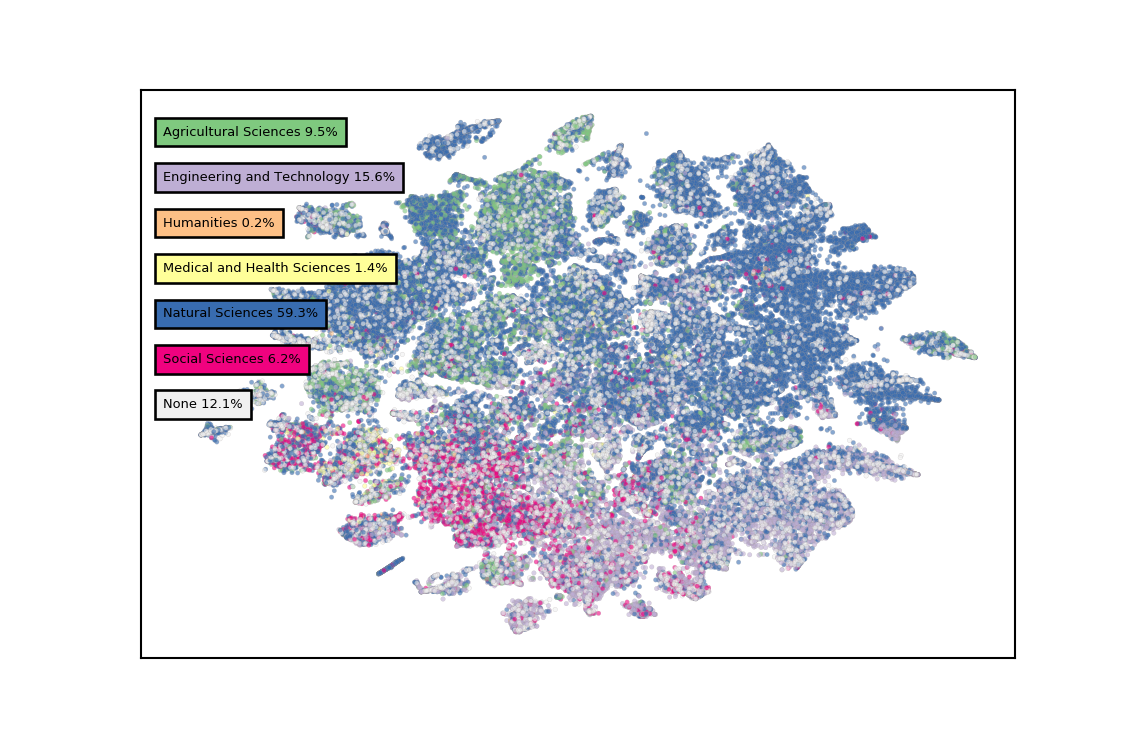
\includegraphics[width=\linewidth]{images/run_665_s_100000_p50_oecds.png}
		\end{figure}
	\end{column}
	\begin{column}{0.33\linewidth}
	\centering \textbf{ Other MCC projects }
	\begin{itemize}
		\item Various systematic review / meta-analysis / topic modelling projects at MCC
		\item Discourse analysis with \textit{Governance} group + parsing of parliamentary archives
	\end{itemize}
	\end{column}	
\end{columns}

\end{frame}





%%%%%%%%%%%%%%%%%%%%%%%%%%%%
%% Website

\begin{frame}{Website}

\url{https://apsis.mcc-berlin.net/scoping}

\end{frame}




%%%%%%%%%%%%%%%%%%%%%%%%%%%%
%% Caveats

\begin{frame}{Caveats}

\begin{block}{Data Collection}<1->

We have a system for downloading queries from databases using our institutional credentials

For external (to MCC) users, you will have to do this step, which includes repetitive clicking, yourself. You can download the appropriate file(s) and upload to our system
\end{block}

\begin{block}{In development}<2->
	
	This is lots of pieces of work tied together, written as a side-project to my PhD. I like improving it, and adding more features, but it sometimes breaks or changes
	
\end{block}


\end{frame}

\begin{frame}{Features}

\begin{itemize}
	\item Managing queries
	\item Screening/tagging documents across author teams
	\item Comparison of coder ratings
	\item Topic modelling
\end{itemize}

\end{frame}

%%%%%%%%%%%%%%%%%%%%%%%%%%%%%%%%%%%%%%%%%%%%%%%%%%%%% 
%% Structure of tool

\begin{frame}{Structure}
	\begin{center}
	\def\yspace{1.5cm}
	\resizebox{0.9\linewidth}{!}{
		\begin{tikzpicture}[node distance=3cm]
		\node<1-> (P) [startstop] {Project};
		\node<1-> (placeholder) [placeholder, right of=P, node distance=8cm] {};
		\node<1-> (placeholder) [placeholder, left of=P, node distance=8cm] {};
		
		% Put users in project
		\node<2-> (U) [startstop, below of=P, node distance=3cm, xshift=-8cm] {User};
		\draw<2-> [arrow] (P) -- (U);
		
		%Do query
		\node<3-> (Q) [startstop, right of=U, node distance=5cm] {Query};
		\draw<3-> [arrow] (U) -- (Q);
		\draw<3-> [arrow] (P) -- (Q);	
		\node<3-> (D) [startstop, below of=Q, node distance=5cm] {Doc};
		\draw<3-> [arrow] (P) -- (Q);
		\draw<3-> [arrow] (D) -- (Q);
		
		% Set up categories and docrels
		\node<4-> (C) [startstop, right of=Q, node distance=2cm, yshift=-1.5cm] {Category};
		\node<4-> (R) [startstop, left of=Q, node distance=5cm, yshift=-3cm] {Relevance};
		\draw<4-> [arrow] (C) -- (Q);
		\draw<4-> [arrow] (R) -- (Q);
		\draw<4-> [arrow] (R) -- (U);
		\draw<4-> [arrow] (P) -- (C);
		
		
		% Go through docs
		\node<5-> (D1) [startstop, right of=D, node distance=0.15cm,yshift=-0.15cm] {Doc};
		\node<5-> (D2) [startstop, right of=D1, node distance=0.15cm,yshift=-0.15cm] {Doc};
		\draw<5-> [arrow] (D) -- (R);
		\draw<5-> [arrow] (D) -- (C);
		%\node<3-> (Presentation) [startstop, right of=Analysis, node distance=6cm] {Presentation};
		
		% Terms
		\node<6-> (Te) [startstop, right of=D2, node distance=9.7cm] {Term};
		\draw<6-> [darrow] (D2) -- (Te);
		
		% Intro topic model
		\node<7-> (M) [startstop, right of=Q, node distance=10cm] {Model};
		\node<7-> (Top) [startstop, right of=Q, node distance=6cm, yshift=-2.5cm] {Topic};
		\draw<7-> [arrow] (M) -- (Q);
		\draw<7-> [arrow] (M) -- (Top);
		
		% doctop, topterm
		\draw<8-> [arrow] (Top) -- (D);
		\draw<8-> [arrow] (Top) -- (Te);
		
		\end{tikzpicture}
	}
\end{center}
\end{frame}

\begin{frame}{Summary}

\begin{center}
	\def\yspace{1.5cm}
	\resizebox{0.9\linewidth}{!}{
		\begin{tikzpicture}[node distance=3cm]
		\node (Data) [startstop] {Data Collection};
		\node (Analysis) [startstop, right of=Data, node distance=6cm] {Analysis};
		\node (Presentation) [startstop, right of=Analysis, node distance=6cm] {Outputs};
		
		\node (WoS) [process, below of=Data, node distance=1.8cm, xshift=-2cm] {WoS};
		\node (Scopus) [process, below of=WoS, node distance=\yspace] {Scopus};
		\node (IPCC) [process, below of=Scopus, node distance=\yspace, fill=orange!10] {IPCC};
		\node (Consolidation) [io, right of=Scopus, node distance=3.5cm] {Consolidation};
		
		\node (Manual) [label, below of=Analysis, node distance=1.8cm, xshift=-1.2cm] {Manual};
		\node (Automatic) [label, below of=Manual, node distance=4.5cm] {Automatic};
		
		
		\node (Review) [process, below of=Analysis, node distance=1.8cm, xshift=1cm] {Systematic Review};
		\node (Scientometric) [process, below of=Review, node distance=\yspace, fill=orange!10] {Scientometric Analysis};
		\node (Text) [process, below of=Scientometric, node distance=\yspace, fill=orange!10] {Other Text Analysis};
		\node (Topics) [process, below of=Text, node distance=\yspace] {Topic Modelling};
		
		\node (Plots) [process, below of=Presentation, node distance=1.8cm, xshift=0cm, fill=orange!10] {Plots};
		\node (Tables) [process, below of=Plots, node distance=\yspace] {Tables};
		\node (Online) [process, below of=Tables, node distance=\yspace] {Online Explorer};	
		
		\draw [arrow, ->] (Manual) -- (Automatic);
		
		\end{tikzpicture}
	}
\end{center}

Future plans:

\begin{itemize}
	\item collecting and synthesizing data within the platform
	\item using machine learning to predict relevance
	\item packaging and publishing tool for wider use
\end{itemize}

\end{frame}



\begin{frame}{Data extraction - meta-analysis}

	\begin{figure}
		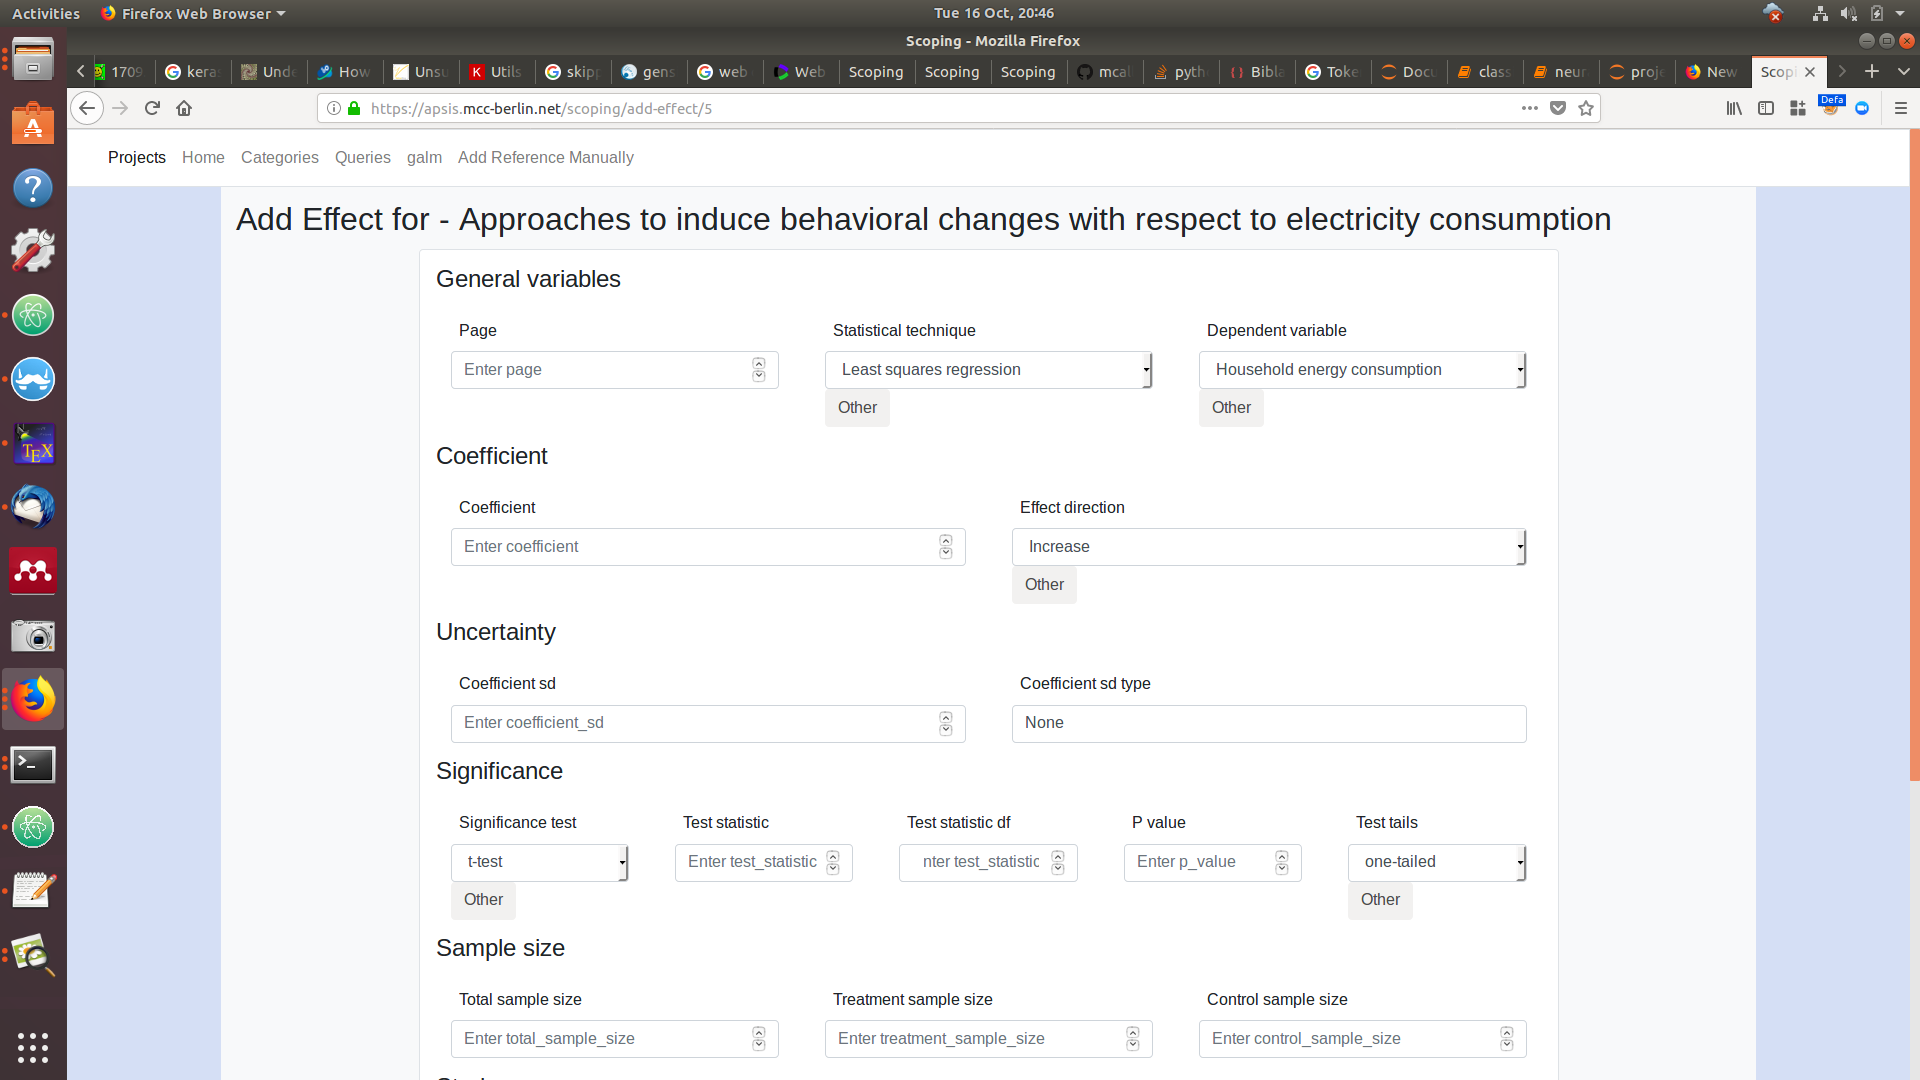
\includegraphics[width=\linewidth]{images/meta.png}
	\end{figure}

\end{frame}



\begin{frame}{Machine learning}

\begin{columns}
	\begin{column}{0.5\linewidth}
		\begin{figure}
			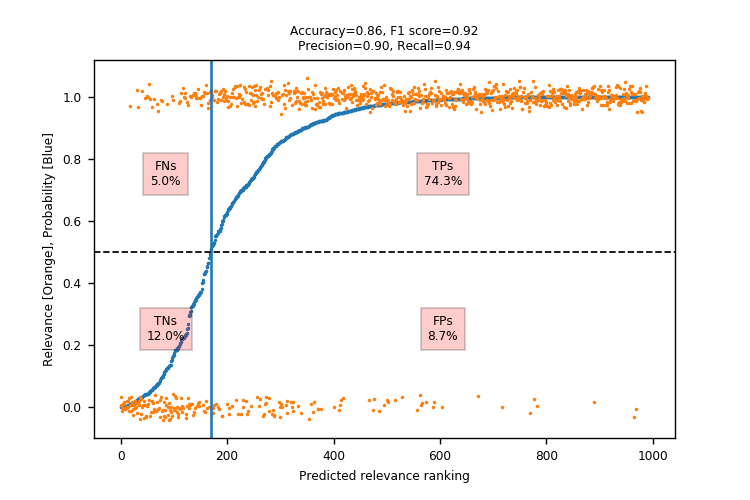
\includegraphics[width=\linewidth]{images/example.png}
		\end{figure}
	\end{column}

	\begin{column}{0.5\linewidth}
		\begin{figure}
				\animategraphics[width=0.8\linewidth]{2}{images/anim/nn_pseudo_active-}{0}{49}
		\end{figure}
	\end{column}
\end{columns}

\end{frame}





\begin{frame}{References}

\scriptsize

Email: \url{callaghan@mcc-berlin.net}

Code: \url{https://github.com/mcallaghan/tmv} (You can raise ``issues'' there)

\medskip

Documentation: \url{https://github.com/mcallaghan/tmv/wiki/Scoping-Documentation} (fairly comprehensive but out of date in \today)

\medskip

\bibliography{/home/max/ownCloud/applications/pubs/mypubs}
\end{frame}


\end{document}